\chapter{Trabalhos relacionados}
\label{chapter:mãos robóticas antropomórficas}

\section{Introdução}

A área da manipulação robótica apresenta inúmeros desafios, particularmente em tarefas que envolvem preensão precisa e troca física de objetos, tanto entre robôs como entre robôs e seres humanos. Nestes contextos, a configuração e natureza da extremidade manipuladora desempenham um papel crucial na eficácia da interação. Para alcançar níveis mais elevados de destreza, flexibilidade e adaptabilidade, o uso de mãos robóticas antropomórficas tem-se revelado uma abordagem promissora. No entanto, estas soluções implicam desafios significativos, desde a conceção e fabrico até à complexidade do controlo, devido ao elevado número de graus de liberdade e à redundância cinemática associada.

Paralelamente, a integração de sensores de contacto é essencial para dotar as mãos robóticas de perceção tátil, permitindo-lhes detetar interações físicas com o ambiente ou entre os próprios dedos. Esta capacidade é fundamental para melhorar o controlo em tempo real, garantir uma manipulação mais segura e possibilitar a implementação de estratégias adaptativas baseadas na perceção sensorial.

Este capítulo apresenta uma análise de diferentes mãos robóticas antropomórficas, incluindo soluções comerciais e plataformas \textit{open-source}, com o objetivo de fundamentar a seleção do modelo adotado neste projeto. Adicionalmente, é feita uma revisão das principais tecnologias de sensores de contacto, culminando na escolha dos mais adequados para integração na mão desenvolvida.


\section{Mãos Robóticas Antropomórficas}

O desenvolvimento de mãos robóticas antropomórficas tem sido alvo de grande interesse na comunidade científica e industrial, devido ao seu potencial para executar tarefas complexas de manipulação com maior destreza e versatilidade. Estas mãos procuram reproduzir, de forma funcional, algumas das capacidades da mão humana, beneficiando de um elevado número de graus de liberdade e de uma estrutura mecânica inspirada na anatomia biológica. 

Esta secção apresenta e analisa diferentes soluções de mãos robóticas antropomórficas existentes, tanto comerciais como \textit{open-source}, com o objetivo de identificar características relevantes para o projeto em desenvolvimento.

\subsection{Soluções comerciais}

Existem várias mãos robóticas antropomórficas disponíveis comercialmente, desenvolvidas com foco na destreza, robustez e integração em ambientes industriais ou de investigação. Estas soluções oferecem alto desempenho, mas geralmente implicam custos elevados, com valores que podem ultrapassar os 10 000€, o que as torna menos acessíveis para projetos académicos ou de prototipagem. Nesta subsecção são apresentadas algumas das opções disponíveis no mercado, como a Oceantrix Hand e a Agile Hand.

\subsubsection{OceanTrix Hand}

A OceanTrix Dexterous Hand (Figura \ref{fig:oceantrix}) é uma mão robótica de sétima geração que apresenta uma arquitetura mecânica com 6 graus de liberdade (DOF), permitindo movimentos coordenados e versáteis dos dedos, adequados para tarefas complexas de manipulação.

O sistema de atuação é totalmente elétrico, utilizando motores de alto desempenho encapsulados em componentes metálicos de grau aeronáutico (alumínio AL6061), o que assegura robustez estrutural e resistência a ambientes exigentes.

A mão incorpora 13 sensores táteis distribuídos estrategicamente nos dedos, proporcionando \textit{feedback} sensorial detalhado que permite um controlo em malha fechada e uma interação sensível com objetos de diferentes formas e texturas. No entanto, esta característica é opcional.

Em termos de integração, a OceanTrix Dexterous Hand é compatível com interfaces de comunicação RS485 e CAN, suportando protocolos como Modbus-RTU. A programação e controlo podem ser realizados através de linguagens como Python e C, oferecendo flexibilidade para integração em diversos sistemas robóticos.

A compatibilidade mecânica com manipuladores específicos não é diretamente indicada nas fontes disponíveis. No entanto, a utilização de interfaces mecânicas padrão e a flexibilidade de comunicação sugerem que a integração com manipuladores existentes é possível, desde que sejam realizadas as adaptações necessárias\cite{oceantrix}.

\begin{figure}[H]
    \centering
    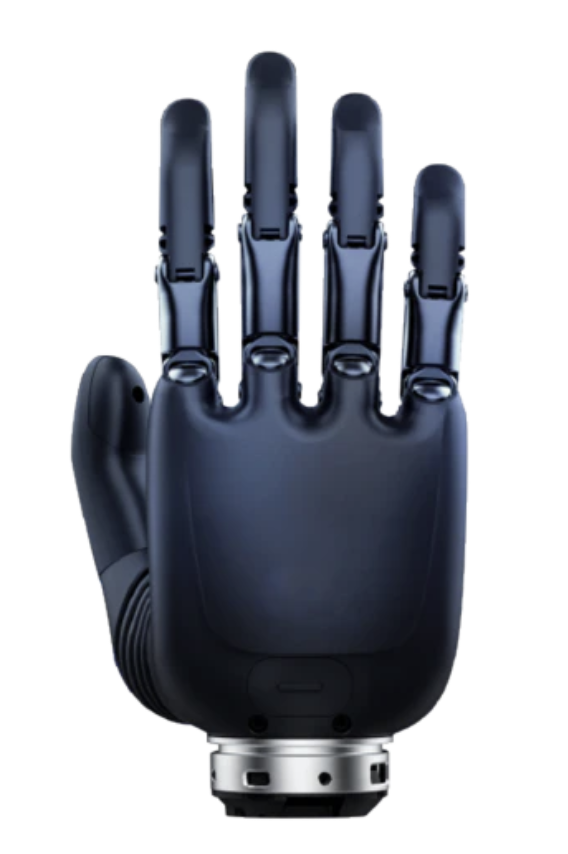
\includegraphics[height=6cm]{figs/chapter2/oceantrix.png}
    \caption{OceanTrix Hand desenvolvida pela  OceanTrix Robotics\cite{oceantrix}.}
    \label{fig:oceantrix}
    
\end{figure}



\subsubsection{Agile Hand}

A \textit{Agile Hand} (Figura \ref{fig:agile}), desenvolvida pela Agile Robots SE, é uma mão robótica antropomórfica com 15 a 16 graus de liberdade, distribuídos por 20 articulações, permitindo movimentos complexos e precisos. Cada dedo é modular e atuado por motores elétricos integrados, capazes de gerar até 10 N de força na ponta dos dedos e velocidades de até 360°/s. A mão incorpora sensores de torque e posição em todas as articulações, permitindo controlo em malha fechada com conformidade ativa. É compatível com manipuladores que seguem a norma ISO 9409-1-50-4-M6 e oferece suporte a C++, Python e ROS, com comunicação a 1 kHz por protocolo proprietário\cite{agile}.

\begin{figure}[H]
    \centering
    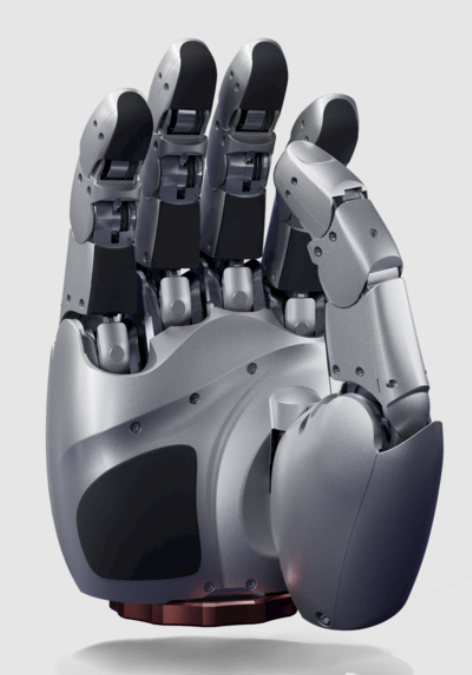
\includegraphics[height=6cm]{figs/chapter2/agile.png}
    \caption{Agile Hand desenvolvida pela Agile Robots SE \cite{agile}.}
    \label{fig:agile}
    
\end{figure}


\subsection{Soluções \textit{open-source}}

As mãos robóticas \textit{open-source} surgem como alternativas acessíveis e personalizáveis às soluções comerciais, especialmente em contextos de investigação e desenvolvimento. Entre as suas principais vantagens destacam-se o baixo custo, a flexibilidade de modificação e a comunidade ativa de utilizadores e desenvolvedores, que facilita a partilha de conhecimento e melhorias contínuas. No entanto, estas soluções apresentam também desvantagens, como a menor robustez mecânica, limitações em precisão e desempenho, e falta de suporte técnico especializado, o que pode representar um desafio em aplicações industriais exigentes.

Para este projeto, a escolha de construir uma mão robótica \textit{open-source} revela-se mais vantajosa, uma vez que será utilizada em contexto de investigação e desenvolvimento, onde a possibilidade de realizar modificações estruturais e funcionais é essencial. Para além disso, a natureza aberta do projeto permite uma maior adaptabilidade aos requisitos específicos da aplicação.


\subsubsection{HRI Hand}

A HRI Hand \cite{Park2020} (Figura \ref{fig:imagem1}) é uma mão robótica antropomórfica \textit{open-source} desenvolvida para atuar como \textit{end-effector} em manipuladores robóticos. Esta mão possui 15 graus de liberdade (sendo apenas 6 juntas ativas),
distribuídos entre os 5 dedos, com cada dedo controlado por um motor linear dedicado, enquanto o polegar utiliza dois motores adicionais para realizar movimentos de abdução e adução. A mão utiliza um mecanismo subatuado baseado num sistema de duas barras articuladas (\textit{four-bar linkage}, ilustrada na figura \ref{fig:imagem2}), permitindo que as articulações \ac{PIP} e \ac{DIP} sejam movidas de forma dependente a partir do motor que controla a articulação \ac{MCP}.

\begin{figure}[h]
    \centering
    \begin{subfigure}[b]{0.45\textwidth} 
        \centering
        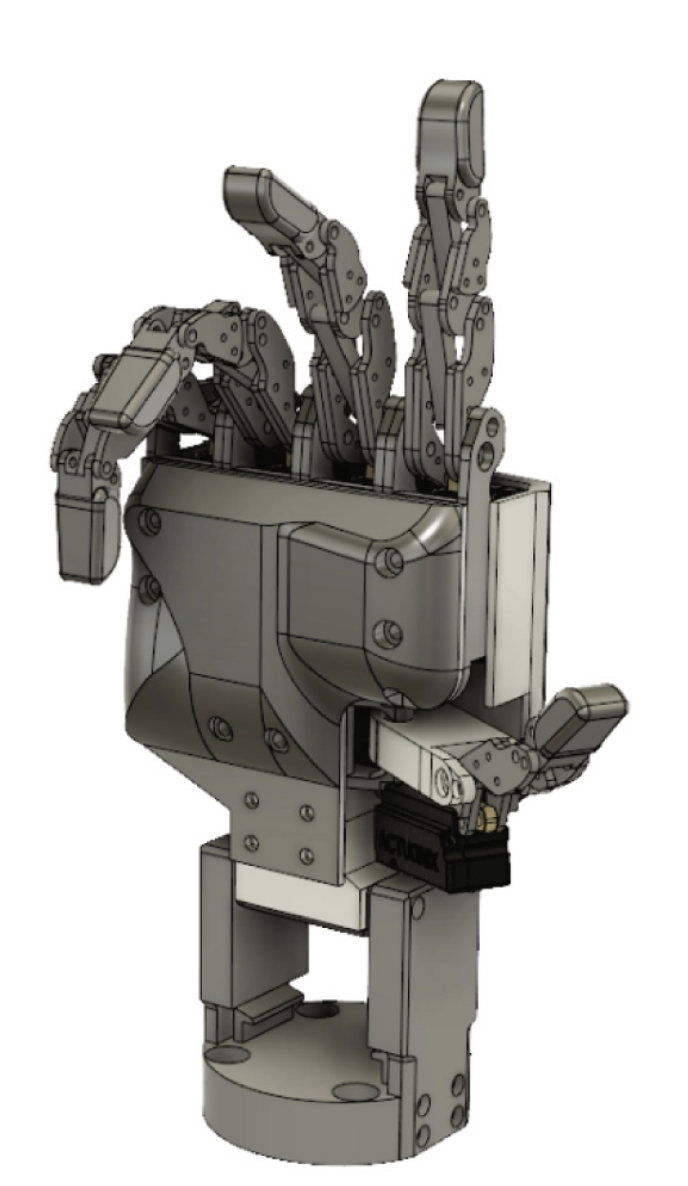
\includegraphics[height=5cm,width=3cm]{figs/chapter2/hri.png}
        \caption{HRI Hand desenvolvida por Park, et al. \cite{Park2020}.}
        \label{fig:imagem1}
    \end{subfigure}
    \hfill
    \begin{subfigure}[b]{0.45\textwidth} 
        \centering
        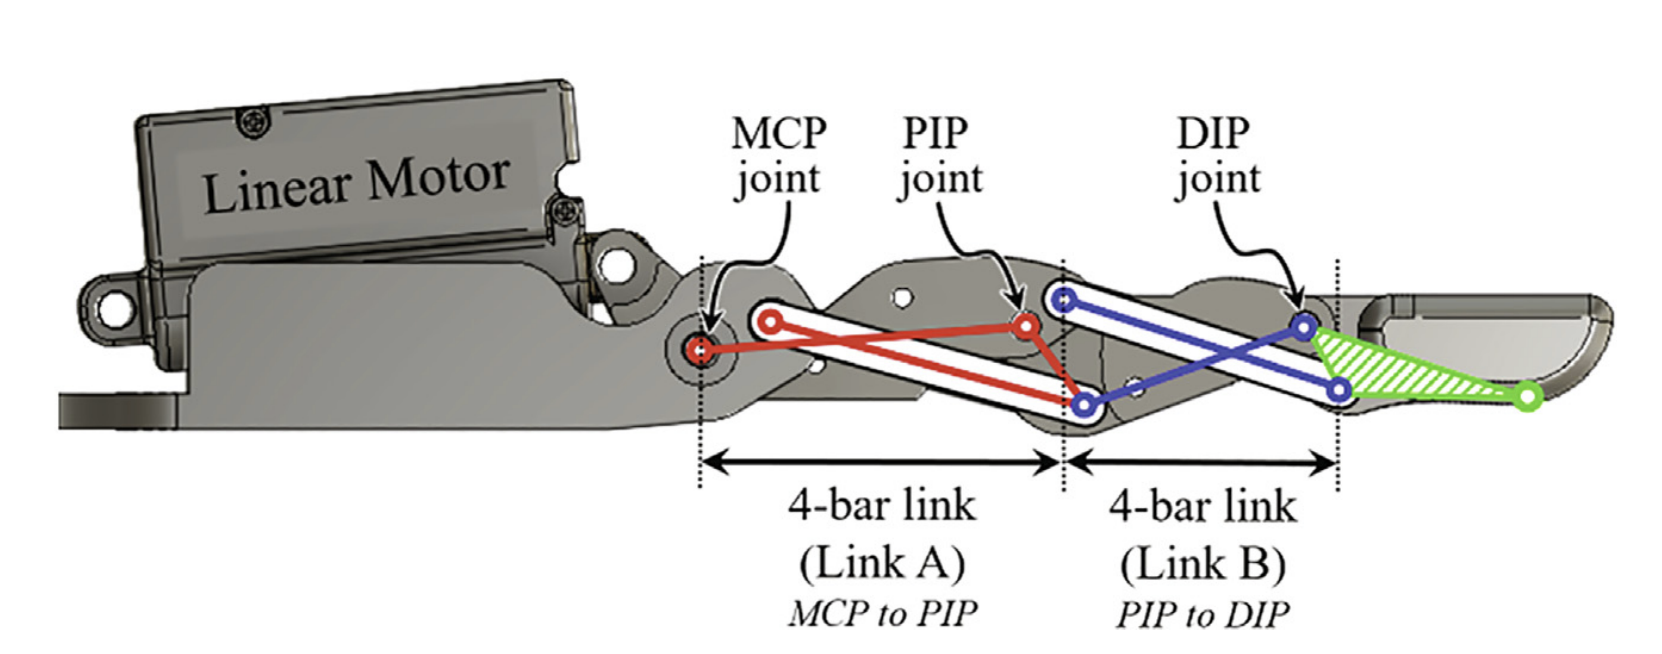
\includegraphics[height=3cm,width=\textwidth]{figs/chapter2/four-bar linkage.png}
        \caption{Sistema de \textit{four-bar linkage} desenvolvida na HRI Hand \cite{Park2020}.}
        \label{fig:imagem2}
    \end{subfigure}
    \caption{Mão HRI e seu mecanismo}
    \label{fig:hri}
\end{figure}

Em termos de compatibilidade de software, a HRI Hand é totalmente integrada com o \ac{ROS} e segue a norma ISO 9409-1-50-4-M6, garantindo compatibilidade com diversos manipuladores robóticos, como o UR3.


\subsubsection{Robot Nano Hand}

A Robot Nano Hand \cite{Nano} (Figura \ref{fig:nano}) é uma mão robótica antropomórfica \textit{open source}, concebida para replicar o tamanho e os movimentos de uma mão humana adulta, oferecendo um total de 11 graus de liberdade. 

A sua estrutura inclui 4 dedos independentes e 1 polegar parcialmente opositor, com cada dedo capaz de realizar movimentos de flexão e laterais, garantindo uma ampla gama de gestos. O sistema de atuação é baseado no uso de tendões, que percorrem os dedos e são controlados por servomotores.

A mão conta também com uma câmara Raspberry Pi V2 integrada na palma, o que a torna adequada para aplicações em visão computacional, incluindo reconhecimento de gestos e análise de objetos. O controlo é gerido por um NVIDIA Jetson Nano Development Kit, um dispositivo robusto que suporta algoritmos de inteligência artificial, como redes neuronais para classificação de imagens e segmentação de objetos.
Embora projetada como uma solução autónoma, com os servos incorporados diretamente na estrutura e um servo adicional que fornece rotação no eixo de inclinação para o conjunto da mão, o design modular da Robot Nano Hand permite adaptações que podem facilitar a sua integração com manipuladores robóticos ou outros sistemas robóticos.

\begin{figure}[H]
    \centering
    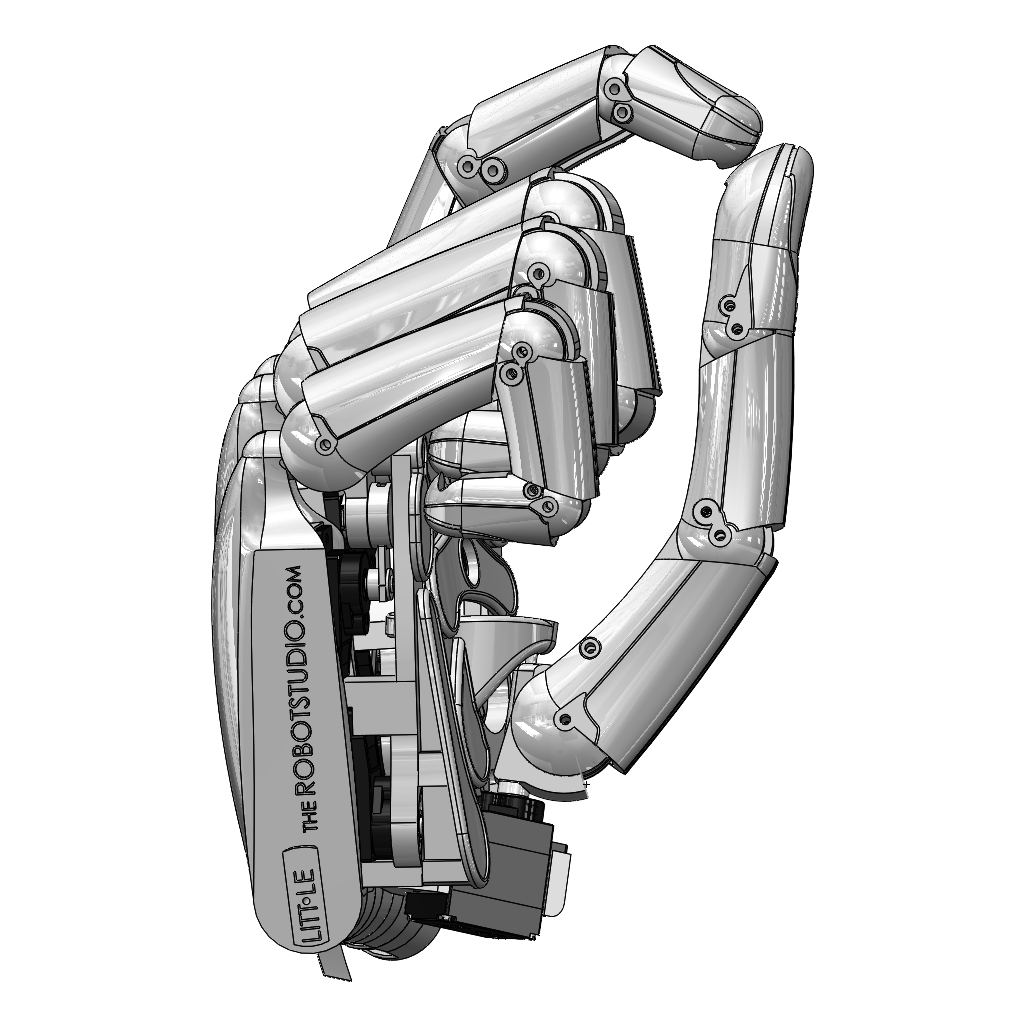
\includegraphics[height=6cm,keepaspectratio]{figs/chapter2/nano.png}
    \caption{Robot Nano Hand desenvolvida por The Robot Studio\cite{Nano}.}
    \label{fig:nano}
    
\end{figure}


\subsubsection{Alaris Hand}

A Alaris Hand \cite{Nurpeissova2021} (Figura \ref{fig:alaris}) é uma mão robótica antropomórfica \textit{open source}, concebida para reproduzir as funcionalidades e movimentos de uma mão humana. 
Este dispositivo apresenta um total de 6 graus de liberdade, permitindo movimentos versáteis dos dedos, que incluem flexão, extensão e manipulação de objetos. 
O sistema de atuação baseia-se em atuadores lineares miniaturizados, acoplados a mecanismos de quatro barras acionados por transmissões de parafuso sem-fim e cremalheira, dispensando o uso de cabos que simulem tendões artificiais. 
Este método garante um controlo eficaz das articulações e proporciona uma força de preensão robusta.
Além disso, a Alaris Hand está equipada com sensores de posição que monitorizam os movimentos articulares em tempo real. 

\begin{figure}[H]
    \centering
    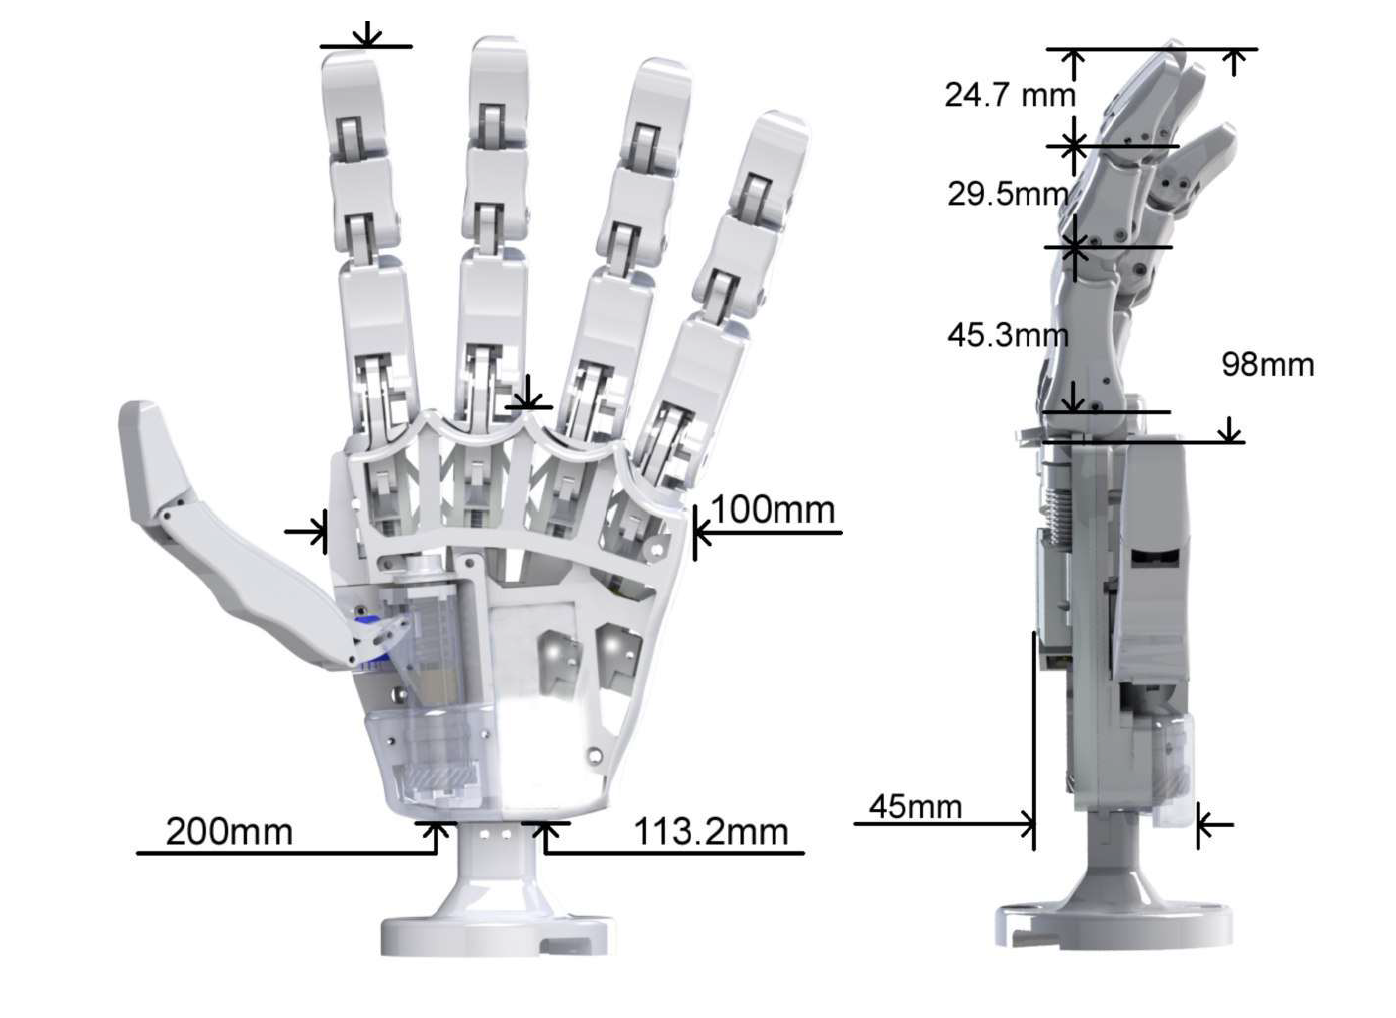
\includegraphics[height=6cm,keepaspectratio]{figs/chapter2/alaris.png}
    \caption{Alaris Hand desenvolvida por Nurpeissova, et al.\cite{Nurpeissova2021}}
    \label{fig:alaris}
    
\end{figure}


\subsubsection{LEAP Hand}

A LEAP Hand \cite{shaw2023leaphand} (Figura \ref{fig:leap_hand})é uma mão robótica antropomórfica de baixo custo, comparado com as soluções comerciais, projetada para aplicações em \textit{machine learning}. 
Esta mão possui 4 dedos e um total de 16 graus de liberdade, com um mecanismo inovador de abdução-adução que mantém todos os graus de liberdade disponíveis em diversas posições das articulações, o que contribui para a sua alta agilidade.
O método de atuação utiliza motores diretos Dynamixel, o que proporciona resistência a torques elevados e aumenta a durabilidade em tarefas de manipulação prolongada.

No que diz respeito aos sensores, a LEAP Hand é capaz de integrar sensores externos para teleoperação ou aprendizagem, mas não possui sensores embutidos nativamente. 
Em termos de software, ela é compatível com diversas plataformas, incluindo \ac{ROS}, Python e C++, além de oferecer um simulador baseado no Isaac Gym e Pybullet, o que permite a realização de experiências de simulação para o mundo real (\textit{sim2real}).

A LEAP Hand é projetada para ser modular e facilmente reparável, utilizando peças impressas em 3D e componentes disponíveis no mercado. A sua compatibilidade com manipuladores robóticos inclui braços como o UR5, o que amplia as suas aplicações em investigação e desenvolvimento.

\begin{figure}[H]
    \centering
    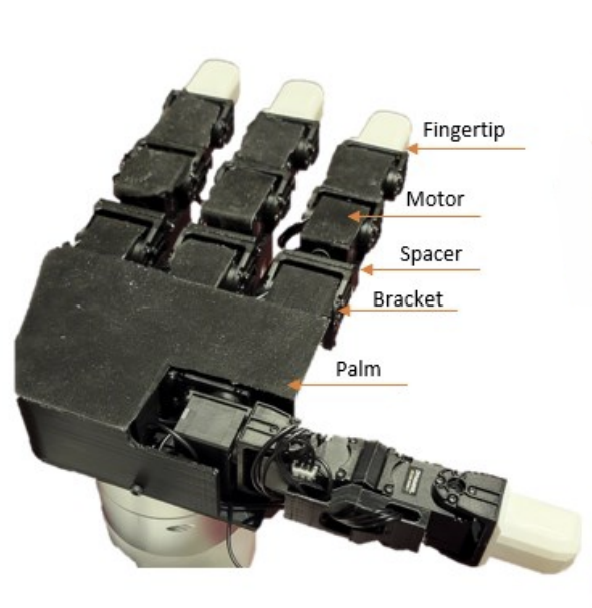
\includegraphics[height=5cm,keepaspectratio]{figs/chapter2/leap_hand.png}
    \caption{Leap Hand desenvolvida por Shaw, et al.\cite{shaw2023leaphand}}
    \label{fig:leap_hand}
    
\end{figure}


\subsection{Seleção da mão a construir}

Após a análise comparativa das diferentes mãos robóticas open-source disponíveis, sumarizada na Tabela~\ref{tab:comparacao_maos}, optou-se pela LEAP Hand~\cite{shaw2023leaphand} como a solução mais adequada para replicação e adaptação no âmbito deste projeto. Esta decisão fundamenta-se principalmente no seu design de construção simples, baseado em servomotores em vez de sistemas de tendões, o que reduz a complexidade mecânica, facilita a montagem e minimiza potenciais pontos de falha.

\begin{table}[H]
    \centering
    \resizebox{\textwidth}{!}{
    \begin{tabular}{l l l l l l}
        \toprule
        \textbf{Modelo} & \textbf{DoF} & \textbf{Atuação} & \textbf{Sensores} & \textbf{Compatibilidade com manipulador} & \textbf{Software} \\
        \midrule
        HRI Hand & 6 & Motores Lineares & Nenhum & UR3 & ROS \\
        Robot Nano Hand & 11 & Tendões & Câmera & Não mencionado & Não mencionado \\     
        Alaris Hand & 6 & Tendões & Posição & Não & Não mencionado \\     
        LEAP Hand & 16 & Servomotores & Posição & UR5 & ROS / Python / C++ / simulação \\
        \bottomrule
    \end{tabular}
    }
    \caption{Comparação entre diferentes mãos robóticas open-source}
    \label{tab:comparacao_maos}
\end{table}

Apesar da sua simplicidade, a LEAP Hand oferece um elevado número de graus de liberdade (16 DoF), superior à maioria das alternativas analisadas, permitindo uma manipulação mais versátil. A presença de sensores de posição integrados garante um controlo eficaz dos movimentos articulares, fator essencial para aplicações em tarefas complexas de manipulação.

Adicionalmente, destaca-se a sua compatibilidade com o sistema ROS, bem como com linguagens de programação como Python e C++, o que proporciona uma plataforma de desenvolvimento acessível e extensível. A possibilidade de integração com manipuladores como o UR5 reforça ainda mais a sua aplicabilidade prática. Por fim, o seu design modular e totalmente imprimível em 3D permite uma manutenção económica e favorece alterações e melhorias iterativas durante o desenvolvimento.



\section{Sensores de Contacto}

A percepção tátil desempenha um papel vital ao permitir que mãos robóticas interajam com o ambiente de forma adaptativa, imitando as capacidades da mão humana.
Esta tecnologia é essencial em áreas como a robótica industrial, onde é necessária uma manipulação precisa, e a aprendizagem por reforço, que se beneficia do \textit{feedback} do mundo real para melhorar o desempenho robótico.

Ao longo dos anos foram propostas diversas tecnologias para sensores táteis, sendo as mais relevantes, no contexto deste trabalho, os sensores baseados em tecnologia magnética, polímeros condutivos e materiais piezoresistivos. Esta secção abordará as principais características e aplicações destas tecnologias em mãos robóticas, destacando as suas vantagens e limitações.

Apesar dos avanços, apenas um número limitado dessas tecnologias tem sido implementado com sucesso em plataformas robóticas reais. Algumas empresas já produzem sensores táteis para aplicações robóticas, como o sensor de ponta de dedo BioTac da SynTouch (ilustrado na figura \ref{fig:biotac})  \cite{Biotac12}. No entanto, estes sensores continuam a apresentar custos elevados e, frequentemente, requerem a integração com outras tecnologias para otimização do desempenho.

\begin{figure}[H]
    \centering
    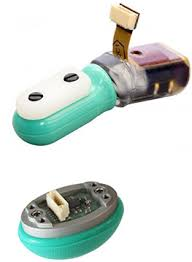
\includegraphics[height=6cm,keepaspectratio]{figs/chapter2/biotac.jpeg}
    \caption{Sensor Biotac desenvolvido pela SynTouch \cite{Biotac12}.}
    \label{fig:biotac}
    
\end{figure}

\subsection{Sensores baseados em Tecnologia Magnética}

Os sensores baseados em tecnologia magnética têm ganho bastante destaque na área da robótica tátil devido à sua elevada precisão, ausência de desgaste e boa durabilidade. Estes sensores destacam-se também por permitirem a deteção de forças sem contacto físico direto com o sensor, o que os torna especialmente interessantes para aplicações em ambientes adversos.

Filmes magnéticos flexíveis, como os apresentados por Jamone, et al. \cite{Jamone2015} (esquema de funcionamento do sensor presente na figura \ref{fig:imagem4}) e  Yan, et al.\cite{Yan2021}, consistem numa camada de elastómero incorporando partículas magnéticas e sensores de efeito Hall colocados abaixo dessa camada. Esta configuração permite medir forças normais e de cisalhamento com elevada sensibilidade, sendo particularmente útil para aplicações em superfícies curvas. No entanto, este tipo de sensor tende a saturar em forças superiores a 4 N, o que limita a sua utilização em tarefas que envolvem forças mais intensas.

\begin{figure}[H]
\centering
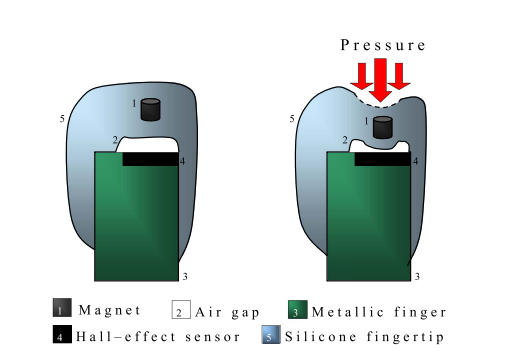
\includegraphics[height=6cm,keepaspectratio]{figs/chapter2/sensor_hall.png}
\caption{Sensor com filme magnético flexível desenvolvido por Jamone, et al. \cite{Jamone2015}.}
\label{fig:imagem4}
\end{figure}



Outra abordagem promissora é o uso de \textit{magneto-elastomer composites}, que combinam materiais elásticos com partículas magnéticas dispersas de forma controlada. Estes sensores, como os utilizados nos trabalhos de Kawasetsu et al. \cite{Kawasetsu2018} (Figura \ref{fig:imagem5}), mostram boa sensibilidade mesmo em contactos rápidos e com elevada aceleração, para além de apresentarem resposta estável a forças contínuas. Contudo, o processo de fabrico pode ser complexo, o que pode implicar maiores custos e limitações em termos de flexibilidade geométrica.

\begin{figure}[H]
\centering
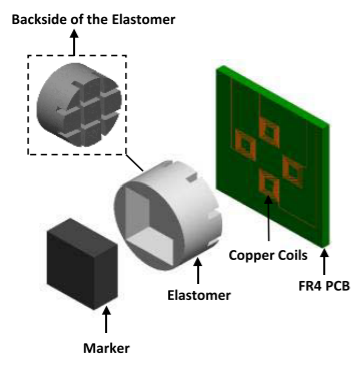
\includegraphics[height=6cm,keepaspectratio]{figs/chapter2/magneto-elastomer.png}
\caption{Composição do sensor desenvolvido por Kawasetsu et al. \cite{Kawasetsu2018}.}
\label{fig:imagem5}
\end{figure}

Os sensores magnetoresistivos representam uma alternativa particularmente robusta, sendo eficazes mesmo em condições adversas como altas temperaturas, humidade ou ambientes com poeiras. O sensor desenvolvido por Alfadhel et al.\cite{Alfadhel2016} utiliza uma estrutura em espiral com materiais magnetoresistivos sensíveis ao campo magnético gerado por uma fonte próxima. Embora a sua robustez seja uma vantagem, estes sensores exigem elevada precisão na montagem e estabilidade dos campos magnéticos externos, o que pode complicar a sua integração em sistemas compactos e móveis \cite{Yang2022}.

\begin{figure}[H]
\centering
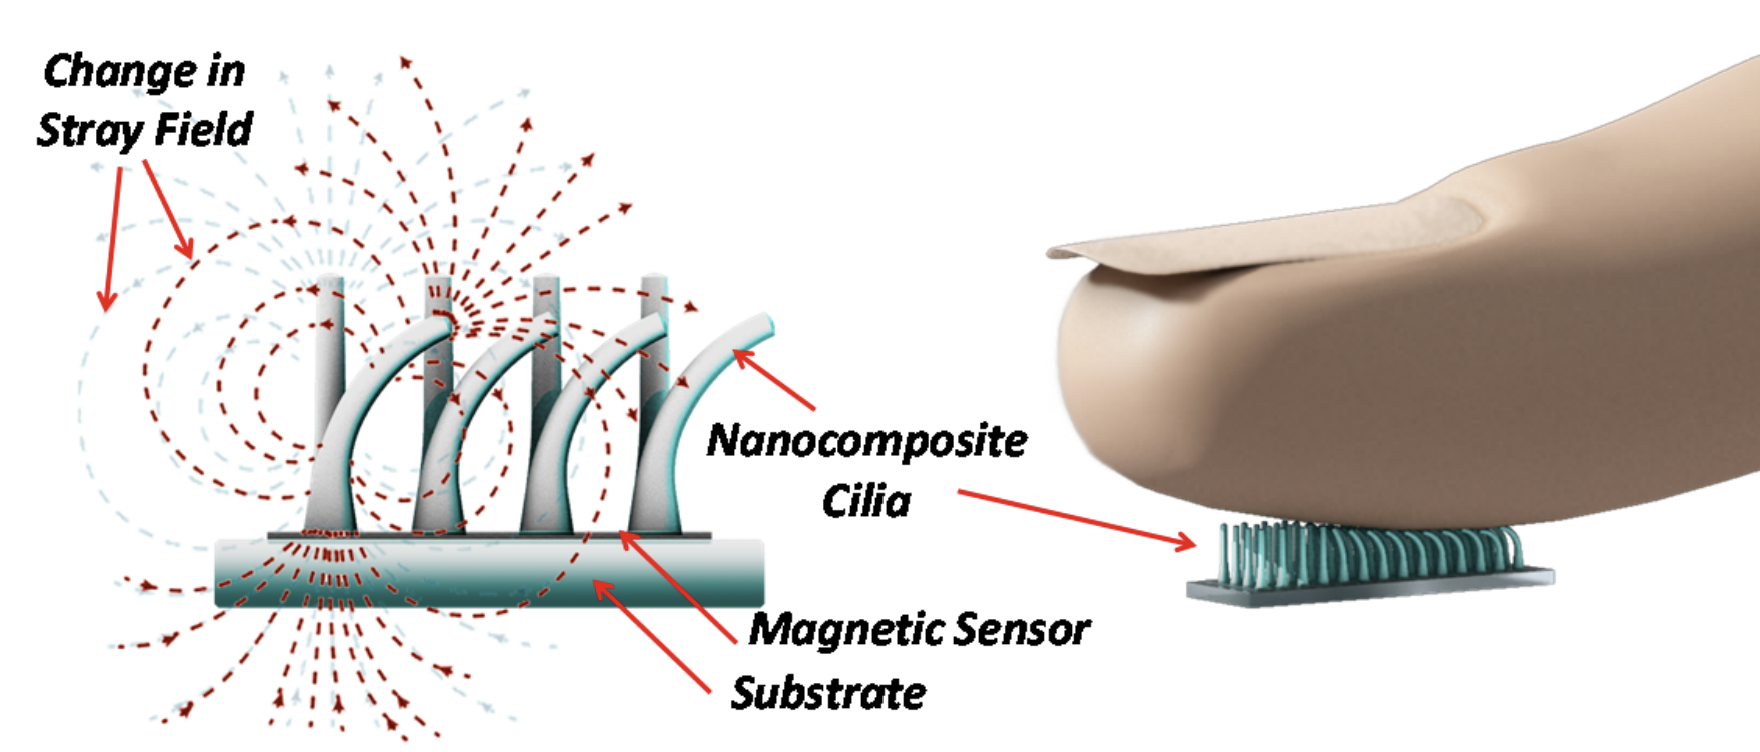
\includegraphics[height=4cm,keepaspectratio]{figs/chapter2/magneto_resistive.png}
\caption{Princípio de operação do sensor baseado em materiais magnetoresistivos \cite{Alfadhel2016}.}
\label{fig:img7}
\end{figure}

Apesar dos desafios, os sensores magnéticos continuam a evoluir e a mostrar grande potencial, sobretudo em aplicações onde a precisão e a resistência a condições ambientais extremas são fundamentais.

\subsection{Sensores baseados em Polímeros Condutivos}

Os sensores baseados em polímeros condutivos têm-se destacado como soluções promissoras para aplicações táteis em sistemas robóticos, sobretudo pela sua leveza, flexibilidade e facilidade de adaptação a superfícies irregulares. Estes dispositivos exploram a variação das propriedades elétricas de materiais condutivos em resposta a deformações mecânicas, permitindo a detecção eficiente de toque e pressão.

Entre as principais abordagens, destacam-se os sensores piezoresistivos, que se baseiam na alteração da resistência elétrica com a aplicação de pressão. São dispositivos de baixo custo e integração simples, adequados para superfícies complexas, como demonstrado em \cite{Canavese2014, Stassi2014}. Contudo, apresentam limitações em termos de precisão, resposta não linear e durabilidade.

Os sensores piezoelétricos, por sua vez, utilizam materiais como o \ac{PVDF}, capazes de gerar sinais elétricos sob estímulos dinâmicos. São valorizados pela elevada sensibilidade, leveza e flexibilidade \cite{Yin2023, Seminara2012}, sendo eficazes na deteção de vibrações e forças variáveis. No entanto, não são apropriados para medições de forças estáticas e requerem circuitos de condicionamento de sinal mais complexos.

Adicionalmente, os sensores triboelétricos operam com base na eletrificação por contato, sendo capazes de gerar sinais elétricos de forma autossuficiente, sem necessidade de alimentação externa. Trabalhos recentes \cite{Zhong2023, Tao2022} demonstram o seu bom desempenho em ambientes adversos. Ainda assim, enfrentam desafios associados à fragilidade mecânica, complexidade de fabrico e sensibilidade a fatores ambientais.

% \begin{figure}[H]
%     \centering
%     \begin{subfigure}[b]{0.45\textwidth} 
%         \centering
%         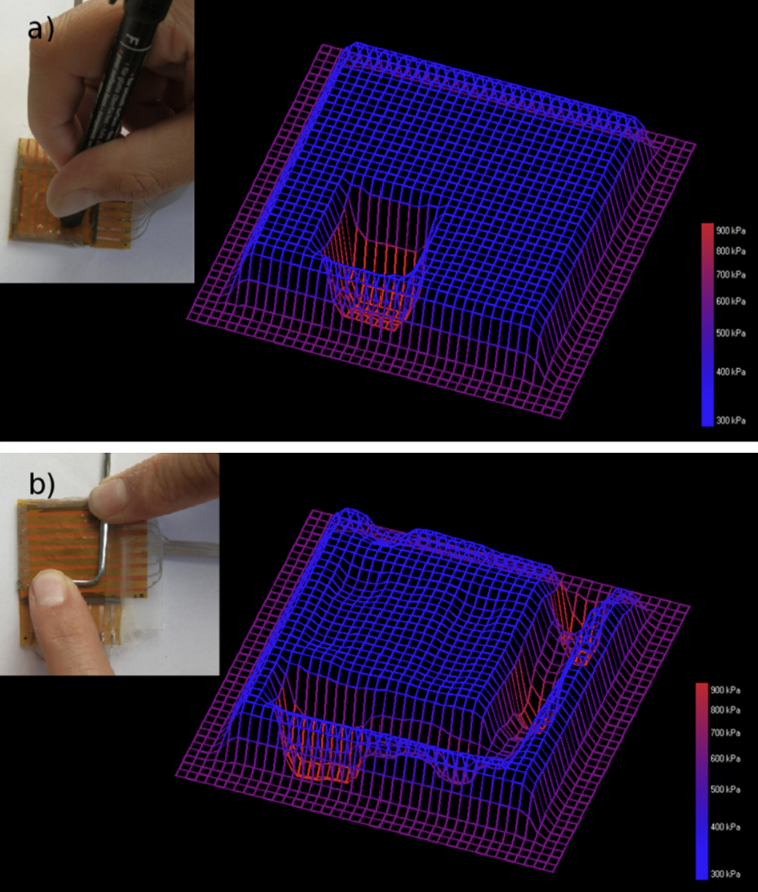
\includegraphics[height=4cm,keepaspectratio]{figs/chapter2/testes.png}
%         \caption{Testes realizados com o sensor desenvolvido em \cite{Canavese2014}.}
%         \label{fig:imagem7}
%     \end{subfigure}
%     \hfill
%     \begin{subfigure}[b]{0.45\textwidth} 
%         \centering
%         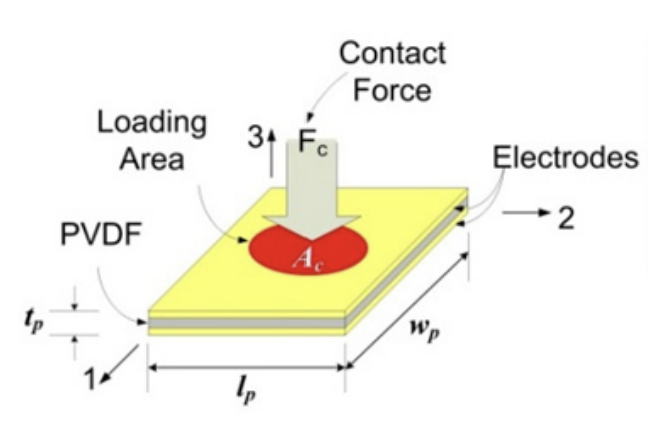
\includegraphics[height=3cm,keepaspectratio]{figs/chapter2/pvdf.png}
%         \caption{Estrutura de um sensor baseado em \ac{PVDF}.}
%         \label{fig:imagem6}
%     \end{subfigure}
%     \caption{Sensores baseados em materiais piezoresistivos}
%     \label{fig:img8}
% \end{figure}


\subsection{Sensores baseados em Materiais Piezoresistivos}

Os sensores baseados em materiais piezoresistivos têm sido amplamente utilizados em aplicações de sensoriamento tátil, especialmente no domínio da robótica, devido à sua elevada sensibilidade à aplicação de forças e pressões. O seu funcionamento baseia-se na variação da resistência eléctrica resultante de deformações mecânicas, permitindo medições precisas e localizadas.

Um exemplo representativo desta tecnologia são os sensores de resistência sensível à força (\acp{FSR}), que combinam um design compacto e robusto com uma elevada adaptabilidade a superfícies curvas e complexas, como as encontradas em mãos robóticas \cite{Ke2019, Lu2023}. Estas características tornam-nos particularmente adequados para sistemas de deteção tátil de baixo custo e fácil integração.

Entre as principais vantagens dos sensores piezoresistivos destacam-se o custo reduzido de produção, a leveza, a flexibilidade e a possibilidade de personalização da sensibilidade em função dos requisitos da aplicação \cite{Stassi2014}. Para além disso, a simplicidade do seu princípio de funcionamento facilita a integração com circuitos eletrónicos de leitura e controlo.

No entanto, estes sensores apresentam também algumas limitações. A sua precisão é, por vezes, inferior à de outras tecnologias sensoriais, e a resposta não linear pode dificultar a calibração. Adicionalmente, a durabilidade e a estabilidade da resposta ao longo do tempo podem ser comprometidas, especialmente em aplicações sujeitas a esforços repetidos ou prolongados \cite{Ke2019}.

% \begin{figure}[H]
%     \centering
%     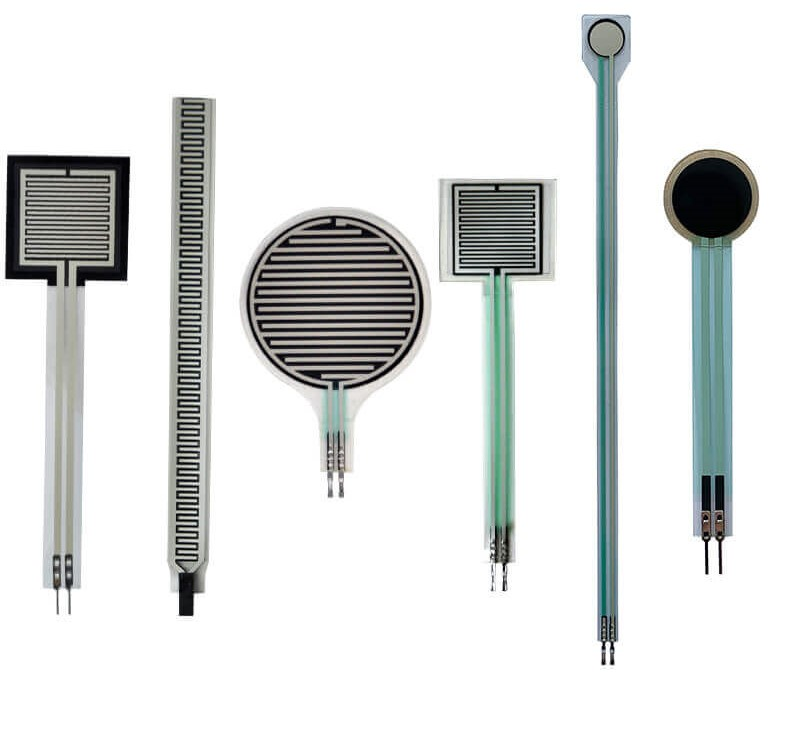
\includegraphics[height=4cm]{figs/chapter2/fsr.jpg}
%     \caption{Sensores \ac{FSR} desenvolvidos pela Interlink.}
%     \label{fig:img9}
    
% \end{figure}


\subsection{Escolha dos sensores a incorporar no projeto}

A seleção dos sensores táteis para o presente projeto foi fundamentada numa análise comparativa entre as diferentes tecnologias disponíveis, com base em critérios como princípio de funcionamento, vantagens técnicas e limitações práticas. A Tabela~\ref{tab:comparacao_sensores} apresenta uma síntese dos principais tipos de sensores considerados.

\begin{table}[H]
    \centering
    \resizebox{\textwidth}{!}{%
    \begin{tabular}{|l|p{5cm}|p{5cm}|p{5cm}|}
        \hline
        \textbf{Tipo de Sensor} & \textbf{Princípio de Funcionamento} & \textbf{Vantagens} & \textbf{Desvantagens} \\
        \hline
        \textbf{Magnético} & Deteta variações em campos magnéticos sem contacto físico direto & Elevada precisão, ausência de desgaste mecânico, boa durabilidade & Custo mais elevado, suscetibilidade a interferência magnética, maior complexidade \\
        \hline
        \textbf{Polímero Condutivo} & Condutividade elétrica varia com a deformação mecânica do material & Elevada sensibilidade, flexibilidade, leveza & Menor durabilidade, sensibilidade a fatores ambientais, resposta lenta \\
        \hline
        \textbf{Piezoresistivo (FSR)} & Resistência elétrica diminui com o aumento da pressão aplicada & Baixo custo, fácil integração, formato compacto e flexível & Resposta não linear, menor precisão, vida útil limitada \\
        \hline
    \end{tabular}%
    }
    \caption{Comparação entre diferentes tipos de sensores táteis}
    \label{tab:comparacao_sensores}
\end{table}

Com base na análise comparativa realizada, os sensores piezoresistivos do tipo \ac{FSR} foram selecionados como a solução mais adequada para o projeto em desenvolvimento. Esta decisão fundamenta-se num conjunto de fatores que favorecem a sua aplicação em contextos de robótica tátil, nomeadamente em mãos robóticas.

Em primeiro lugar, destaca-se a sua estrutura fina, leve e flexível, que permite uma integração eficiente em superfícies curvas, como as pontas dos dedos e a palma da mão robótica. Para além disso, os \acp{FSR} oferecem um equilíbrio vantajoso entre desempenho e acessibilidade económica.

Adicionalmente, o seu design compacto e a simplicidade de integração com os sistemas eletrónicos permitem reduzir significativamente a complexidade de implementação, fator particularmente relevante em projetos com restrições de espaço físico, como é o caso da LEAP Hand \cite{shaw2023leaphand}.



\section{Conclusão}

Ao longo deste capítulo foram analisadas várias opções tecnológicas com vista à definição da arquitetura sensorial do projeto. Numa primeira fase, avaliou-se um conjunto de mãos robóticas antropomórficas, tanto comerciais como open-source, com o objetivo de selecionar uma solução adequada aos requisitos de integração tátil. Desta análise resultou a escolha da LEAP Hand\cite{shaw2023leaphand}, cuja estrutura modular, dimensões compactas e compatibilidade com sensores externos a tornam particularmente apropriada para o presente projeto.

De seguida, procedeu-se ao estudo comparativo de diferentes tecnologias sensoriais, nomeadamente sensores baseados em princípios magnéticos, polímeros condutivos e materiais piezoresistivos. A avaliação teve em consideração fatores como sensibilidade, facilidade de integração e viabilidade económica.

Com base nesta análise, foram selecionados sensores piezoresistivos do tipo \ac{FSR}, devido ao seu formato compacto, baixo custo, facilidade de aplicação em superfícies curvas e capacidade de resposta adequada aos requisitos de deteção tátil em mãos robóticas.

Em suma, as decisões tomadas relativamente à mão robótica e à tecnologia sensorial asseguram uma base sólida para o desenvolvimento do sistema de perceção tátil, alinhando-se com os objetivos técnicos e funcionais definidos para o projeto.

